%%%%%%%%%%%%%%%%%%%%%%%%%%%%%%%%%%%%%%%%%%%%%%%%%%%%%%%%%%%%%%%%%%%%%%%%%%%%%%%%
%2345678901234567890123456789012345678901234567890123456789012345678901234567890
%        1         2         3         4         5         6         7         8

\documentclass[letterpaper, 10 pt, conference]{ieeeconf}  % Comment this line out if you need a4paper

%\documentclass[a4paper, 10pt, conference]{ieeeconf}      % Use this line for a4 paper

\IEEEoverridecommandlockouts                              % This command is only needed if 
                                                          % you want to use the \thanks command

\overrideIEEEmargins                                      % Needed to meet printer requirements.

% See the \addtolength command later in the file to balance the column lengths
% on the last page of the document

% The following packages can be found on http:\\www.ctan.org
\usepackage{graphics} % for pdf, bitmapped graphics files
\usepackage{caption}
\usepackage{subcaption}
\usepackage{standalone}
\usepackage{tikz}
\usepackage{tikzscale}
\usetikzlibrary{calc}
%\usepackage{epsfig} % for postscript graphics files
%\usepackage{mathptmx} % assumes new font selection scheme installed
%\usepackage{times} % assumes new font selection scheme installed
%\usepackage{amsmath} % assumes amsmath package installed
%\usepackage{amssymb}  % assumes amsmath package installed

\title{\LARGE \bf
Preparation of Papers for IEEE Sponsored Conferences \& Symposia*
}


\author{David Landry and Alexandre Gari�py}


\begin{document}

\maketitle
\thispagestyle{empty}
\pagestyle{empty}


%%%%%%%%%%%%%%%%%%%%%%%%%%%%%%%%%%%%%%%%%%%%%%%%%%%%%%%%%%%%%%%%%%%%%%%%%%%%%%%%
\begin{abstract}

  abstract

\end{abstract}

%%%%%%%%%%%%%%%%%%%%%%%%%%%%%%%%%%%%%%%%%%%%%%%%%%%%%%%%%%%%%%%%%%%%%%%%%%%%%%%%
\section{INTRODUCTION}


\section{RELATED WORK}


\section{PROBLEM DEFINITION}
\begin{itemize}
    \item Talk about teach and repeat
    \item How teach maps are aquired (point clouds are taken at regular steps)
    \item Why we want to optimize this (loop closure spped, memory for large maps)
\end{itemize}


\section{OUR APPROACH}
\begin{itemize}
  \item Choose elipse of a given shape. We assume that if ICP converges on the
    ellipse, it would converge at any given point inside the ellipse (we need the explain why we made this assumption)

  \item For each point, find the nearest point that doesn't converge with ICP

  \item Create an oriented graph where arcs represents a successful ICP convergence

  \item Find the shortest path in the graph from that converge

\end{itemize}

\begin{figure}[thpb]
  \centering
  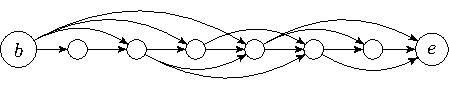
\includegraphics[scale=1.0]{img/unoptimized-graph.pdf}
  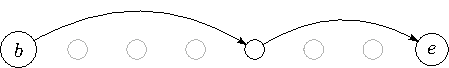
\includegraphics[scale=1.0]{img/optimized-graph.pdf}
  \caption{Optimal node subset using the graph approach}
\end{figure}


\section{EXPERIMENTS}
We can talk about the offline optimisation we did on some dataset.

\begin{figure}
  \caption{Comparison of un-optimized and optimized maps}
\end{figure}


\section{FUTURE WORK}

\begin{itemize}
  \item Experiment with Husky

  \item Multi objective optimization to have an automatic error elipse

  \item handling rotations (3D ellipsoid)

  \item Reoptimisation of the graph

\end{itemize}

\section{CONCLUSION}

\end{document}
